\documentclass[11pt]{amsart}
\usepackage{geometry}                % See geometry.pdf to learn the layout options. There are lots.
\geometry{letterpaper}                   % ... or a4paper or a5paper or ... 
%\geometry{landscape}                % Activate for for rotated page geometry
%\usepackage[parfill]{parskip}    % Activate to begin paragraphs with an empty line rather than an indent
\usepackage{graphicx}
\usepackage{amssymb}
\usepackage{epstopdf}
\usepackage{setspace} 
\usepackage{amsmath}

\DeclareGraphicsRule{.tif}{png}{.png}{`convert #1 `dirname #1`/`basename #1 .tif`.png}

\title{Brief Article}
\author{The Author}
%\date{}                                           % Activate to display a given date or no date
\usepackage{parskip}
\setlength{\parindent}{15pt}

\begin{document}
\begin{spacing}{1.1}
\maketitle
%\section{}
%\subsection{}

\section{Report}

In the previous chapter, we have seen that using a MFCC representation of utterances with regions of silence removed leads to a large improvement in accuracy, time and computational complexity in the performance of DTW algorithm augmented with a  euclidean metric..The main contributing factor behind the large time and computational complexity of  the base line DTW is the \textbf{size} of the time series sequences. The computational cost of a DTW algorithm is $(mn)$ where $m$ and $n$ denote the length of the two time series sequences currently compared. Using longer sequences increases the size of the DTW cost matrix hence resulting into a greater number of computations.

The DTW algorithm on its own  is a domain independent  algorithm that  uses a similarity metric  to  compare  any two sequences through comparison of  their  global trends.  The algorithm  employes dynamic programming to search a space of mapping between the time axis of  the two respective sequences to determine the optimum alignment between them.  The only difference between MFCC-augmented DTW and baseline DTW is the feature extraction stage. In machine learning, feature extraction refers to the pre-processing stage that involves the extraction of new features from a set of raw attributes through a suitable functional mapping. The extraction phase of MFCC features  involves a segmentation of the time series followed by a functional mapping on the segmented windows. The  resultant sequence of  extracted feature vectors has a much smaller length compared to the length of the original sequence. Evident from the  experiments done in the previous chapters, the use mel-cepstrum features extracted on `cleaned' signals not only increases the accuracy of DTW but also reduces the time and computational cost through reduction of dimensionality of the original sequence.

Any time series sequence contains both local and global trends. In some time series datasets[], it has been observed that incorporating the information about these local trends and global shapes in the clustering /classification process does improve the performance of the DTW. The feature extraction methodologies used for their works  are domain and application independent. The MFCC feature extraction  on the other hand, is a domain  and application dependent. This feature extraction process can only be applied to time series sequences corresponding to speech. From a  scientific stand point, it will be interesting to compare and see how well/bad the domain independent methods are to  domain dependent methods. In this chapter, I investigate  an unsupervised methodology that:

\begin{itemize}
\item incorporates  information about local and global trends  in the feature extraction process
\item employs an adaptive DTW that tackles the issue of the large time and computational complexity by moving from working on  time series sequences to  sequences of segmented time-slices. To counter the tradeoff in the decrease  in accuracy, the algorithm is equipped with a kernel function(self-proposed) that is designed to measure the similarity of sub-sequences more accurately than standard euclidean metric by being invariant toward time-dilation and scale.   
\end{itemize}

\section {{Feature extraction}}

\\
The fundamental problem of baseline DTW  is that the numerical value of a data point in a time series sequence is not a complete picture of the data point  in relation to the rest of the sequence. The context such as the position of the points in relation to their neighbours is ignored. To fix  this issue, an alternative  form of DTW know as \epmh{Derivative} DTW is proposed but the fundamental problem with this DTW is that it  fails to detect significant common sub-patterns between two sequences(mainly global trends). Ideally we need to use features that contains information about the overall shapes of the sequences plus the local trend around the points. This allows the DTW to built a complete picture of the data point in relation to the rest of the sequence and hence achieve a better optimal alignment between the two sequences.

For feature extraction, the methodology that I have used  for this setup is based on Xie and Wiltgen's paper[].  Each point in the time series sequence is replaced by a 4 dimensional vector  where the first two features correspond to information regarding the local trends around a point and the last two features reflect the position of that point in the global shape of the sequence.

Definition of local feature given in [] is as follows:
\[ f_{\mbox{local}}(r_i)= (r_i-r_{i-1}, r_i-r_{i+1})\]



The  extraction of global features is constrained by two factors: the features that reflect information about  global trends and  the features must be in the same scaling order  as the local features. Being in the same scale allows them to  be combined with local features. In [] the authors used the following method to extract global features from the time series sequence:
\[ f_{\mbox{global}}(r_i)= (r_i -\sum_{k=1}^{i-1}\frac{r_k}{i-1} , r_i-\sum_{k=i+1}^M \frac{r_k}{M-i})\]


\section{Adaption of DTW}
The feature extraction methodology discussed above results in a time series sequence of vectors where the length of the series is $\|X_n\|-2. $   ($\|X_n\| $ denotes the original length of the time series sequence).  The DTW augmented with these features will still suffer from large time and computational complexity as before. In the MFCC feature extraction, the time series sequence is first segmented into series of frames  of length 20ms. Through appropriate functional mapping, the frames are converted into vectors. Because the length of the resultant sequence of vectors is much smaller than the length of the original time series the size of the  DTW cost matrix is smaller than before. This decreases the time and computational cost associated with each comparison.

Using this as motivation,  the time series of 4d vectors extracted in the previous stage are segmented using windows  of width 10ms.  The number of segmented windows is much smaller than the length of sequences. Thus if we adapt the DTW to work on sequence of frames rather than the time series sequences, we can achieve a large improvement in the time and computational cost  associated in the testing phase. 

The problem now can be shifted to finding  an appropriate kernel that can be used to compute the similarity between two subsequences  of feature vectors while adjusting to the temporal skewness present within the subsequences. Intuitively speaking , we need a kernel that behaves like a DTW on pairs of  subsequences.


The motivation behind the kernel proposed for this problem comes from the polynomial kernel. 
Lets consider the following example.
Let $x$ and $z$ be two dimensional vectors.
Consider the simple polynomial kernel of degree 2  :$k(x,z) = (x^{T}z)^2$ .  This kernel can expressed as :
\begin{eqnarray*}
k(x,z) &= &(x^{T}x')^2\\
&  =& (x_1z_1+x_2z_2)^2\\
&= & x_1^2z_1^2 + 2x_1z_1x_2z_2 + x_2^2z_2^2\\ 
&=& (x_1^2, �2x_1x_2, x_2^2)(z_1^2, �2z_1z_2, z_2^2)^{T}\\
&=& \phi(x)^{T}\phi(z)\\
\end{eqnarray*}
Hence the 2nd order polynomial kernel is equivalent to a corresponding feature mapping $\phi$  that contains terms of order 2. Now, if we generalise this notion then $k(x,z) = (x^{T}z)^M$ contains all monomials of order M. For instance, if x and z are two images, then the kernel represents a particular weighted sum of all possible products of M pixels in the first image with M pixels in the second image.

Now consider the following signals:
\begin{figure}[h!]
  \centering
   
     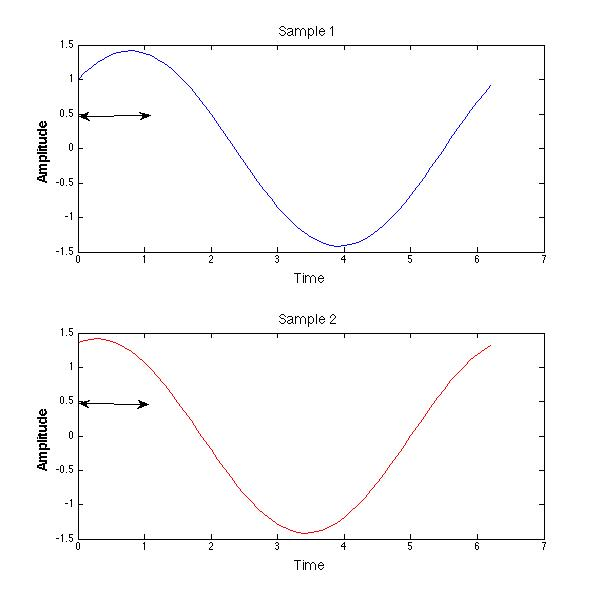
\includegraphics[scale=0.6]{Example1.jpg}
  \caption{Two signals separated by translation}
  
\end{figure}
The signal denoted by the `blue' color is a translation of the signal denoted by the `red' color . From our methodology constructed  so far, each time series point is replaced by a 4-dimensional vector and the resultant  time series sequence of  vectors is segmented using windows of size 10ms. In the example above, lets consider the window spanned by the arrows. 

\begin{figure}[h!]
  \centering
   
     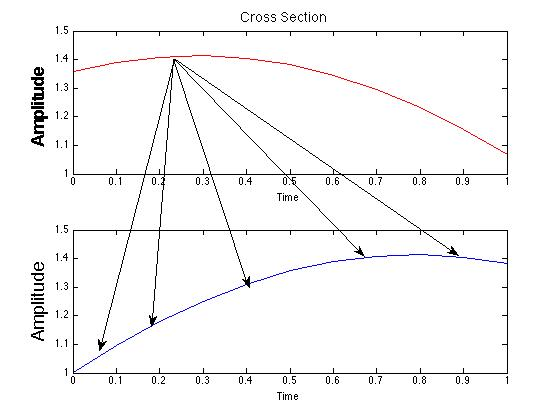
\includegraphics[scale=0.6]{Cross-section.jpg}
  \caption{Two identical subsequences varying in time }
  
\end{figure}
Ideally, we want a metric that takes into account that two similar subsequences may vary in time and speed. We will want to compare the global and local properties associated with a point in one subsequence with the global and local properties of points at  different regions in the second sub-sequence illustrated by figure 2.  Using a euclidean metric in this scenario is inappropriate. The euclidean metric  in this context is identical to  linear time warping where the  two subsequences will be matched based on a linear match of the two temporal dimensions.  In our context, we need a kernel that computes the similarity/distance between two sub-sequences by warping the time axis.  From the earlier  discussion of the polynomial kernel, we have seen that if we consider the generalised case then $k(x,z) = (x^{T}z)^M$  represents a particular weighted sum of all possible products of M time series points in the first sub-sequence with M time series points in the second subsequence here $x$ and $z$ represent respective subsequences. Using this as motivation I propose the following metric:.
\[ k(x,z) = <\sum_{i=1}^{n}x_i, \sum_{j=1}^{n}z_j>\]
where $n$ denotes the length of the window and $x_i$ s and$z_i$ represents the 4-dimensional features associated point i in the first sequence and point j in the second sequence.

For a windows of size 3, this kernel  metric representation can be expanded and   expressed as :

\begin{eqnarray*}
k(x,z) &= &<\sum_{i=1}^{3}x_i, \sum_{j=1}^{3}z_i>\\
&  =& (x_1+x_2+x_3)(z_1+z_2+z_3)\\
&= & <x_1z_1>+<x_1z_2>+<x_1z_2>+<x_2z_1>+<x_2z_2> +<x_2z_3>+......\\ 
\end{eqnarray*}

From above expression, we can see  that the proposed kernel corresponds to a sum of all possible dot products of pairs belonging to the set
$\{(x_iz_i) | x_i\in \mbox{seq1}, z_i \in \mbox{seq2}\}$. Thus  we match each feature vector in 1 subsequence with all feature vectors in the 2nd sequence.

It is easy to check that the kernel I propose here is in fact a valid kernel:
\begin{itemize}
\item K(x,z)= K(z,x) $\Rightarrow $the function is symmetric.
\item The kernel satisfies Mercer's theorem : K(x,z) =$\phi(x)^T\phi(x)$
where  the feature mapping corresponds to $\phi(y) = \sum_{i=1}^{3}y_i$. 
\end{itemize}



%Kernel functions must be continuous, symmetric, and most preferably should have a positive (semi-) definite Gram matrix. Kernels which are said to satisfy the Mercer's theorem are positive semi-definite, meaning their kernel matrices have no non-negative Eigen values. The use of a positive definite kernel insures that the optimization problem will be convex and solution will be unique.


\end{spacing}
\end{document}  